\section{Enumeration Method}

\textbf{Probleme mit Iterator}

\begin{itemize}
	\item Iterator und Collection sind stark gekoppelt
	\item Aufwendiges Lifecycle Management notwendig; Iterator muss Collection überwachen
\end{itemize}

\textbf{Alternative zu Iterator}

Kapsle Iterationslogik über eine Collection in eine Enumeration Method der Collection, die ein Command Object mit der Verarbeitungslogik entgegennimmt.

Auch als Internal Iterator bekannt, jedoch nur selten berücksichtigt.

\begin{figure}[H]
	\centering
	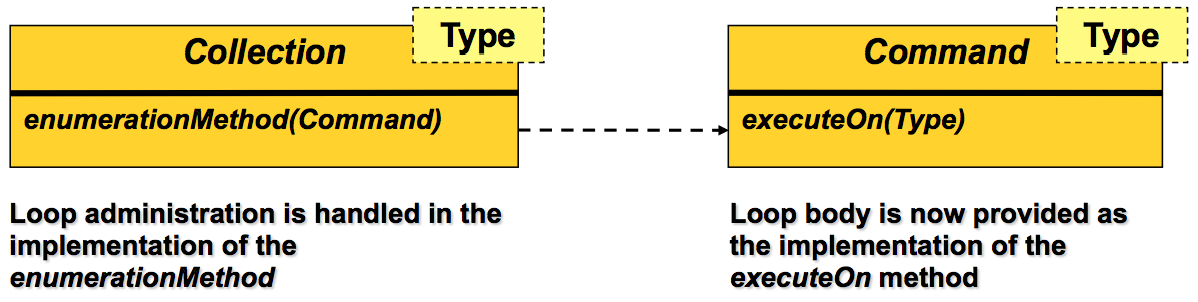
\includegraphics[width=0.9\textwidth]{content/advancedPatterns/enumerationmethod.png}
	\caption{Enumeration Method}
\end{figure}

\textbf{Konsequenzen}

\begin{itemize}
	\item Client ist nicht für die Verwaltung eines Iterators zuständig
	\item Synchronisation kann für die gesamte Traversierung gewährleistet werden, statt nur pro Zugriff
	\item Führt zum Teil zu unnötig viel Code und Verschmutzung des Namespaces da viele Command Objekte benötigt werden
	\item Kann u.U. zur Verwirrung führen; ``zu abstrakt''
\end{itemize}


\section{State Patterns}

\textbf{Objects for States}

Siehe GoF State Pattern

\textbf{Methods for States}

Stelle jeden Zustand als Tabelle von Methoden oder Funktionen dar, die über diese Tabelle aufgerufen werden.

\textbf{Konsequenzen}

\begin{itemize}
	\item Das Verhalten eines Objekts kann vollständig innerhalb der Klasse definiert werden (als private Methods); keine ``Verzettelung'' wie bei Objects for States
	\item Methodenaufrufe werden zusätzlich umgeleitet; Performanceeinbussen
	\item Teilen von Verhalten zwischen unterschiedlichen Zuständen ist sehr einfach
	\item Vertehen der Klasse wird schwieriger, da das genaue Verhalten in einem Zustand durch den Leser aufgeschlüsselt werden muss
	\item Nur geeignet in Sprachen, die das referenzieren und auflösen von Methoden einfach unterstützen. z.B. C++, Scala, Ruby im Gegensatz zu Java
\end{itemize}

\textbf{Collections for States}

Gruppiere Objekte im selben Zustand in Collections sodass der State durch dazugehörigkeit zu einer Collection repräsentiert wird. So können z.B. in einem Editor, der mehrere Dateien bearbeitet, alle veränderten Dateien in einer Collection ``changed'' abgelegt werden und alle unveränderten in der Collection ``saved''. Um nun alle Dateien zu speichern kann über alle ``changed'' Dateien iteriert werden, welche anschliessend nach ``saved'' verschoben werden.

\textbf{Konsequenzen}

\begin{itemize}
	\item Aktionen über alle Aktionen eines bestimmten States sind effizient durchführbar
	\item Bei Systemen mit beschränkten Ressourcen kann der Memory Footprint pro Objekt u.U. verringert werden, da der State implizit über die Collectionzugehörigkeit bestummen wird
	\item Es können unterschiedliche Zustandsmodelle auf Objekte angewendet werden, ohne diese zu erweitern
	\item Der Manager bekommt mehr Verantwortung als beim Objects for States Pattern
	\item Das halten von Zustandsabhängigen Daten für die Objekte ist schwieriger
\end{itemize}

